%//==============================--@--==============================//%
\subsection[3.1 Amostragem (\textit{Sampling})]{$\rightarrow$ Amostragem (\textit{Sampling})}
\label{subsec:sampling}

Seja $x(t)$ um sinal arbitrário de energia finita. Supondo que o sinal é amostrado a uma cadência uniforme---a cada $T_S$ segundos---obtém-se, consequentemente, uma sequência de amostras espaçadas por este mesmo intervalo, $\{x(nT_S)\}$. Define-se $T_S$ $[$s$]$ como o período de amostragem, e $f_S \delequal 1/T_S$ como a frequência de amostragem $[$S/s$]$.

\vspace{0.75em}
\noindent Na sua forma geral, o processo resulta em:
$$
    \boxed{ x_s(t) = \sum_{n=-\infty}^{+\infty} x(nT_S)\, p(t-nT_S) }
$$
em que $p(t)$ é a forma do pulso utilizado. Na amostragem ideal, $p(t) \equiv \delta(t)$.

%//==============================--@--==============================//%
\subsubsection[3.1.1 Amostragem instantânea]{$\rightarrow$ Amostragem instantânea (\textit{instantaneous/ideal sampling})}
\label{subsubsec:instantaneous-sampling}
$$
    x_{\delta}(t) = \sum_{n=-\infty}^{+\infty} x(nT_S)\, \delta(t-nT_S) \,\xleftrightharpoons[\mathcal{F}]{}\, X_{\delta}(f) = f_S \sum_{m=-\infty}^{+\infty} X(f-m f_S)
$$

\vspace{-1em}
\begin{theo}[\underline{Teorema da Amostragem} (Teorema de Nyquist-Shannon)]{teo:sampling}\label{teo:sampling}
    Seja $x(t)$ um sinal de energia finita (banda limitada), com frequências não superiores a $W$. Então, este sinal é totalmente descrito através de uma coleção de amostras espaçadas por $1/(2W)$ segundos; sendo perfeitamente reconstruído através destas amostras.

    \vspace{0.5em}
    \noindent A \underline{menor frequência} de amostragem possível que não resulta em \textit{aliasing} é
    $$
        f_S = f_N \delequal 2W
    $$
    denominada por \underline{frequência de Nyquist}. $\pmb{\rightarrow}$ \textbf{Critério de Nyquist:} $f_S \geq f_N$ 

    \vspace{0.75em}
    \noindent \textbf{Nota:} Por vezes é definida uma banda de guarda, e deste modo: $f_S \delequal f_{S0} + B_G$
\end{theo}

\begin{figure}[H]
    \centering
    \begin{minipage}[c]{0.5\textwidth}
        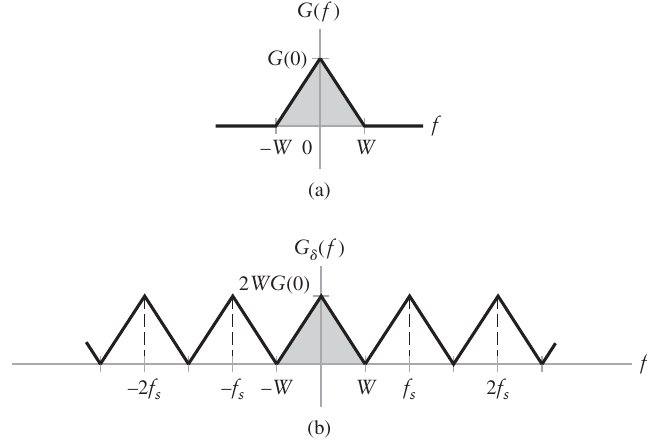
\includegraphics[width = 1\linewidth]{img/digital/sampling/sampling-frequency-domain.png}
    \end{minipage}
    \raisebox{0em}{
    \hspace*{0.5em}\begin{minipage}[c]{0.4\textwidth}
        \caption{(a) Espectro do sinal de banda limitada $g(t)$. (b) Espectro da versão amostrada idealmente, $g_\delta(t)$, a um ritmo de $T_S = 1/(2W)$ (não ocorre \textit{aliasing}).}
        \label{fig:sampling-frequency-domain}
        
        \vspace{-1.5em}
        \begin{theo}[\underline{\textit{Aliasing}}]{def:aliasing}\label{def:aliasing}
            Se o critério de Nyquist não se verificar satisfeito, as cópias adjacentes sobrepõem-se e não é possível discernir um $X(f)$ não ambíguo.
        \end{theo}       
    \end{minipage}}
\end{figure}

\renewcommand*{\thefootnote}{\fnsymbol{footnote}}
\footnotetext[4]{%
    Tomando uma $f_S = 2W$, e assumindo um filtro passa-baixo ideal para a reconstrução do sinal com uma frequência de corte $f_c = f_S/2 = W$, obtém-se a expressão:
    $$
        x(t) = \sum_{n=-\infty}^{+\infty} x\left(\frac{1}{2W}\right)\, \text{sinc}(2W t - n),\quad -\infty < t < +\infty
    $$
    denominada por \textit{interpolation formula}---para reconstruir o sinal $x(t)$ através de uma sequência de valores amostrados $\{x(nT_S)\}$, em que a função sinc($2W t - n$) é a \textit{interpolation function}.
}
\renewcommand*{\thefootnote}{\arabic{footnote}}
%adoro-te :3
%//==============================--@--==============================//%